\chapter{Proposed Protocol}
\section{Considerations}
% Coping with hops, on demand (reactive) or table driven (proactive), (minimise need but use AODV or DSR). 
LoRa packets can only be 256 bytes (due to FIFO buffer size, see official documentation https://www.semtech.com/products/wireless-rf/lora-transceivers/SX1276).
LoRa packet transmit time ranges from 200ms to 1s depending on packet size.\
https://github.com/sudomesh/disaster-radio/wiki/Protocol
\section{Proposal}
% Duty cycles (decided on method [manage per hour])
% Bands (dual band)
% Message types
% PHY layer parameter selection
% Adaptiveness???
% a461331.pdf general collision avoidance
%


\section{Duty Cycle}
\begin{figure}[H]
    \centering
   	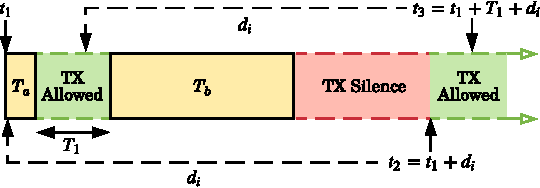
\includegraphics{Figures/duty_cycle_proposed.pdf}
    \caption[Proposed duty cycle enforcement method]{
    Demonstration of proposed method for duty cycle limit enforcement. Unlike \ac{lorawan}'s method the behaviour can vary greatly depending on when transmissions occur and how long they are, therefore this diagram is only a partial representation. It is valid provided there are no transmissions since $t=t_1-d_i$, where $d_i$ is the duty cycle interval (e.g. 3600 seconds). The duty cycle ($d_c$) shown is $\frac{T_a + T_b}{d_i}$. Enforcement is handled as follows. Immediately after the first transmission occurs, the remaining interval allowance is $T_b$ ($T_a+T_b-T_a$). This could be used immediately but, for purposes of demonstration, a short period of silence occurs. Once the transmission of length $T_b$ occurs, the remaining interval allowance is 0 ($T_b - T_b$), therefore the transmitter must be silent until allowance is freed. At $t_2$ a transmission of length $T_a$ would be allowed because for every time unit of a new transmission, the corresponding time unit of $T_a$ would no longer fall in the time interval. A longer transmission would not be allowed until $t_3$ because $T_b$ will not fall outside of the time interval until $T_1$ has elapsed. Note that as $T_a$ is already available the transmission can start $T_a$ before $T_b$ actually falls out of the interval. Therefore at $t_3$ a transmission of $T_a + T_b$ would be allowed (in this case, the full interval limit). The figure is not to scale.    
    }
    \label{fig:proposed_duty_cycle}
\end{figure}

Phy testing has shown that distance cannot be covered by a gateway
Proposed solution is agnostic to routing protocol


Duty cycle:
Can quickly get complicated to understand when dealing with more complex transmission scenarios  (e.g. short send, wait, short send, wait, long send, etc...). However, simple to implement using a linked list, which gets culled when a send needs to occur. Delete old entries and find overlaps with current time - di. Can start sending as soon as the previous transmission started. Though processing intensive, allows predictable scheduling.

